\chapter{Algoritmi randomizzati}
\section{Classificazione}
Gli algoritmi randomizzati sono algoritmi dove eventi casuali influiscono sulla struttura dell'algoritmo stesso: oltre ai dati in ingresso influiscono valori casuali che ne determinano l'evoluzione. Li classifichiamo in due tipi:
\begin{itemize}
    \item \textbf{Las Vegas}
    
    Algoritmi con risultato \textbf{\underline{sicuramente}} corretto in un tempo probabilmente breve %(Quicksort\footnote{Nel quickSort si fanno alcuni passi a caso per aggirare configurazioni sfavorevoli su cui l'algoritmo va lento. Si pensi a quando scegliamo come pivot scegliamo sempre l'elemento massimo (in una sequenza già ordinata il partizionamento va male): se scegliamo il pivot in modo deterministico l'avversario può predisporre i dati nell'array in modo tale che venga scelto dall'algoritmo il pivot desiderato dall'avversario stesso.})
    
    \item \textbf{Monte Carlo}
    
    Algoritmi con risultato \textbf{\underline{probabilmente}} corretto in un tempo sicuramente breve (test di primalità di Miller-Rabin, potrei avere risultati non corretti). Questi algoritmi offrono tuttavia la possibilità di scegliere l'errore con il quale si ottiene il risultato. La probabilità di errore deve essere:
    \begin{itemize}
    	\item arbitrariamente piccola, e matematicamente misurabile.
    \end{itemize}
	Questo ci permetterà di rendere l'errore trascurabile.
\end{itemize}

\section{Test di primalità (inefficiente)}
Consideriamo il seguente test di primalità e valutiamone l'efficienza
\begin{center}
	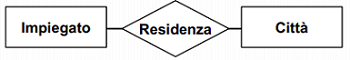
\includegraphics[scale=.61]{images/6.PNG}
\end{center}
\begin{center}
	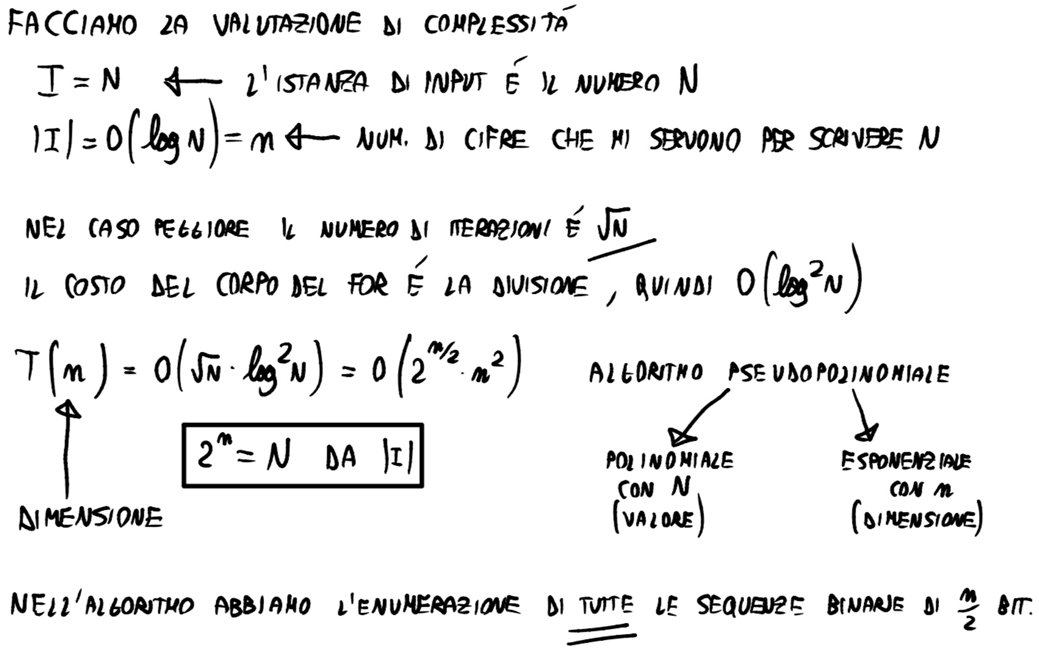
\includegraphics[scale=.7]{images/6bis.PNG}
\end{center}
L'algoritmo è pseudopolinomiale, cioè:
\begin{itemize}
	\item polinomiale rispetto al valore;
	\item \underline{esponenziale rispetto alla dimensione del valore} (non tengo conto solo del numero, ma anche di quanto è grande il numero).
\end{itemize}
Vogliamo un algoritmo più efficiente: introduciamo per questo il test di primalità secondo Miller-Rabin, basato su sequenze casuali.

\section{Test di primalità: algoritmo di Miller-Rabin}
\subsection{Premessa}
Vogliamo testare un intero dispari $N$ su $n$ bit. Se $N$ è dispari allora $N-1$ è pari.
$$
N-1 = 2^{\omega}z
$$
con $z$ dispari e $2^{\omega}$ la più grande potenza di $2$ che divide $N-1$. Vediamo due esempi:
\begin{align*}
	N &= 17 \implies N-1 = 16 = 2^{4} \cdot 1 \Longrightarrow z=1,\omega=4\\
	N &= 21 \implies N-1 = 20 = 2^{2} \cdot 5 \Longrightarrow z=5, \omega =2
\end{align*}
$z$ e $\omega$ ci serviranno nell'algoritmo: si noti che entrambi possono essere trovati in tempo polinomiale in quanto posso dividere un numero per $2$ al massimo $\log_2N$ volte quindi abbiamo un algoritmo polinomiale nel numero di cifre di $N$ ($n = \log_2N$)

\subsection{CN (ma non sufficienti) per il test di primalità} Supponiamo che $N$ sia un numero primo. Si prenda $y$, un intero casuale arbitrario tale che $ 2 \leq y \leq N-1 $ (che prende il nome di \emph{testimone}). Affermiamo che per $N$ valgono le seguenti proposizioni:
\begin{align*}
	\text{P1}:&\text{ } \text{MCD}(N, y) = 1\\\text{P2}:&\text{ } \left(y^z \text{ mod } N = 1\right) \text{ OR } \left(\exists i: 0 \leq i \leq \omega - 1 \text{ t.c. } y^{2^i \cdot z} \text{ mod } N = -1\right)
\end{align*}
Se il numero è primo allora vale sia P1 che P2. In P2 basta che una delle condizioni sia valida. Possiamo usare la veridicità di entrambi i predicati come condizione necessaria per il nostro test di primalità, tuttavia non è sufficiente in quanto esistono numeri composti (pochi) che verificano entrambi i predicati.

\subsection{Lemma di Miller-Rabin (pochi composti verificano le CN)}
Se $N$ è numero composto il numero di testimoni $y$ t.c. $2 \leq y \leq N-1$ che soddisfa i predicati $P1$ e $P2$ è basso, precisamente $< \frac{N}{4}$.
\paragraph{Cioè} Questo significa che se scelgo a caso un testimone $y$ la probabilità che ne scelga uno che rende veri i due predicati è minore della probabilità di scegliere un testimone dove uno dei due predicati è falso.
$$
    \text{P(scegliere $y$ t.c. $P1 \text{ AND } P2 = 1$)} < \frac{\frac{N}{4}}{N-2} < \frac{1}{4}
$$
Facciamo il rapporto tra casi favorevoli e casi possibile: $N-2$ è il numero di casi possibili (scelte possibili tra i testimoni), $\frac{N}{4}$ sono i casi favorevoli (in cui i due predicati sono entrambi soddisfatti).
\paragraph{Quindi} Immaginiamo i seguenti passi per verificare P1 e P2:
\begin{verbatim}
dato N scelgo a caso y in [2, N-1]
allora:
se uno dei due predicati è falso:
    N è certamente composto
se entrambi i predicati sono veri:
    N è composto con probabilità < 1/4, N è primo con probabilità > 3/4
\end{verbatim}
Per ridurre la probabilità posso re-iterare il processo di selezione di $y$. Se ripeto il procedimento $k$ volte scendiamo ad una probabilità 
$ < \frac{1}{4^k} $ che $N$ sia composto. Per avere un'idea  iteriamo il processo trenta volte:
\[k=30 \Longrightarrow \left(\frac{1}{4}\right)^{30} \simeq 10^{-18}\]


\subsection{Algoritmo completo e costo computazionale} 
Scriviamo l'algoritmo completo in pseudo-codice:
\begin{verbatim}
// Controlla la validita' del certificato y (certificato di N composto)
VERIFICA(N, y){
    if (P1 == false OR P2 == false) return 1
    return 0
}
TESTMR(N, k){
    for(i = 0; i < k; i++){
        y = numero a caso in [2, N-1]
        if(verifica(N, y) == 1) return 0    // N sicuramente non è primo
    }
    return 1            // N è primo con probabilità < 1/4^k
}
\end{verbatim}
\begin{itemize}
	\item Il costo di $\text{TESTMR}$ è $k \cdot \text{VERIFICA}$ in quanto si itera la verifica sul singolo testimone per k volte. L'esecuzione $k$ volte riduce la probabilità di errore da $\frac{1}{4}$ a $\left(\frac{1}{4}\right)^k$
	\item \textbf{Calcoli per il primo predicato}. La verifica di $P1$ è il calcolo del $MCD$ quindi si ha costo polinomiale nella dimensione di $N$ tramite l'algoritmo di Euclide.
	\begin{align*}
 		\text{ } \text{MCD}(N, y) = 1
	\end{align*}
	\item \textbf{Calcoli per il secondo predicato}. La verifica di $P2$ richiede il calcolo di potenze
	\begin{align*}\text{ } \left(y^z \text{ mod } N = 1\right) \text{ OR } \left(\exists i: 0 \leq i \leq \omega - 1 \text{ t.c. } y^{2^i \cdot z} \text{ mod } N = -1\right)
	\end{align*}
	La cosa è abbastanza critica perché queste operazioni richiedono tempo esponenziale nella dimensione di $N$. Si pensi che il valore massimo assumibile dall'esponente della $y$ si ha con $i=\omega - 1$, quindi risulta necessario fare $\frac{N-1}{2}$ moltiplicazioni (otteniamo ciò da $N-1=2^\omega z$, la premessa poco avanti) per ottenere il risultato desiderato \[2^{(\omega-1)} \cdot z=\frac{N-1}{2} \Longrightarrow \text{Caso peggiore: } y^{2^{(\omega-1)} \cdot z} = y^{\frac{N-1}{2}} \]
	
	Risolviamo il problema implementando l'\textbf{algoritmo delle quadrature successive} (posto nell'appendice sull'algebra modulare), con cui riduciamo il numero di moltiplicazioni richieste per ottenere una potenza.
\end{itemize}

\clearpage 

\section{Generazione di numeri primi}
\begin{framed}
	\noindent \textbf{Domanda da esame}.
	
	\noindent Illustrare con quale metodo si generano numeri primi grandi in crittografia e spiegare perché tale 	metodo è considerato efficiente.
\end{framed}
Non abbiamo algoritmi propri per la generazione di numeri primi però possiamo seguire il seguente approccio:
\begin{enumerate}
    \item generare un numero casuale
    \item si testa la sua primalità
    \item se questo numero casuale non è \emph{dichiarato} primo si aumenta di due e si ripete da (2)
\end{enumerate}
\paragraph{Densità dei numeri primi sull'asse degli interi} L'algoritmo introdotto conviene perché per un lemma di Gauss sappiamo che il numero di interi primi e minori di un numero dato $N$ tende a:
$$ \longrightarrow{} \frac{N}{\log_eN} \,\,\,\,\text{per }N \to \infty$$
quindi preso un $N$ abbastanza grande sappiamo con quasi certezza che esisterà un primo in un intorno circolare di ampiezza $\log_eN$.

\paragraph{Algoritmo} Scriviamo quindi un algoritmo in pseudocodice:
\begin{verbatim}
PRIMO(n): // n : numero di bit desiderati per il numero primo
    S = sequenza casuale di n-2 bit
    N = 1 S 1 // concatenamento dei bit per avere num. lunghi e sicuramente dispari
    while(TESTMR(N, K) == 0) N += 2
    return N
\end{verbatim}
L'1 come bit più significativo serve per avere un numero sempre elevato (potrei avere sequenze con bit più significativi tutti uguali a 0), l'1 meno significativo mi da certezza che andremo a considerare un numero dispari. Abbiamo quindi TESTMR con complessità O($n^3$), viene ripetuto O($n$) volte quindi in totale l'algoritmo ha complessità: O($n^4$). 


